\documentclass[10pt]{beamer}

\usetheme[progressbar=frametitle]{metropolis}
\usepackage{appendixnumberbeamer}
\usepackage{graphicx}
\usepackage{booktabs}
\usepackage[scale=2]{ccicons}
\usepackage[font=footnotesize,labelfont=bf]{caption}
\usepackage{mwe}

\usepackage{pgfplots}
\usepgfplotslibrary{dateplot}

\usepackage{xspace}
\newcommand{\themename}{\textbf{\textsc{metropolis}}\xspace}

\title{Multivariable Spatial Prediction and Model Validation}
\subtitle{}
% \date{\today}
\date{}
\author{Stefano Fochesatto}

\begin{document}

\maketitle


%http://www.billharlan.com/papers/kriging/kriging.html
\begin{frame}{What is Multivariable Spatial Prediction}
    \begin{itemize}
        \item Methods we have discussed in class offer prediction of one variable at a time.     
        \item Recall,
        \begin{equation*}
            \hat{y}(s_0) = \sum_{i = 1}^n \lambda_i y(s_i) 
        \end{equation*}
        \begin{itemize}
            \item Ordinary Kriging; $\lambda_i$'s are constrained by relative distances.
            \item Universal Kriging; $\lambda_i$'s are also constrained by trends and covariates. 
        \end{itemize}
        \vfill
        \item For Universal Kriging we found $\lambda_i$'s by minimizing MSPE,
        \begin{equation*}
            MSPE = \mathbb{E}\left[\left( Y(s_0) - \sum_{i = 1}^n \lambda_i y(s_i)\right)^2 \right],
        \end{equation*}
        by the following constraint (lagrange multipliers), 
        \begin{equation*}
            \bar{\lambda}^TX = x_0^T.
        \end{equation*}
        \item To find the $\bar{\lambda}$ using Least\-Squares it was necessary to estimate a variogram for $Y$. 
    \end{itemize}
\end{frame}


%http://www.u.arizona.edu/~donaldm/homepage/my_papers/MathGeology_29_1997_685-704.pdf
%Noel Cressie book Cokriging section
\begin{frame}{What is Multivariable Spatial Prediction}
    \begin{itemize}
    \item What if we don't have $x_0$ where we want to predict $s_0$, but we still have secondary data that has information?!
    \vfill
    %% Separate the sum, note the lambda as a conversion. 
    \item Cokriging methods follow analogously in derivation; and allow us to directly use existing spatial correlations from secondary-data,
        \begin{equation*}
            \hat{y}(s_0) = \sum_{i = 1}^n\lambda_{i} y_1(s_i)   +  \sum_{j = 1}^k \lambda_{j} y_2(s_j) + \dots
        \end{equation*} 
    \item In solving for $\lambda_{i}$ and $\lambda_{i}$ using Least\-Squares it becomes necessary to estimate variograms and cross\-variograms for all $Y_i$. 
    \end{itemize}
\end{frame}


%% Insert slide about cross variograms. 

\begin{frame}{What is Multivariable Spatial Prediction}
    \begin{itemize}
    \item The goal is the spatial prediction of multiple variables simultaneously. 
    \vfill
    \item Multivariable Spatial Prediction is an extension of Cokriging. 
    \vfill
    \item 'It is shown that the cokriging predictor for one variable at a time is
    identical to the predictor of that same variable in the multivariable predictor.' $\-$ Ver Hoef $\&$ Cressie (1993)
    \vfill
    \item The constraints for solving for the weights change when cokriging a variable at a time. 
    \end{itemize}
\end{frame}

\begin{frame}{Kriging Overview}
    \begin{itemize}
        \item 'The truth of the matter is, when someone says 'kriging' I kind of blend it all together in my mind.' - M. Short.
        \item same tbh
    \end{itemize}
\end{frame}


\begin{frame}{Kriging Overview}
    \begin{center}
    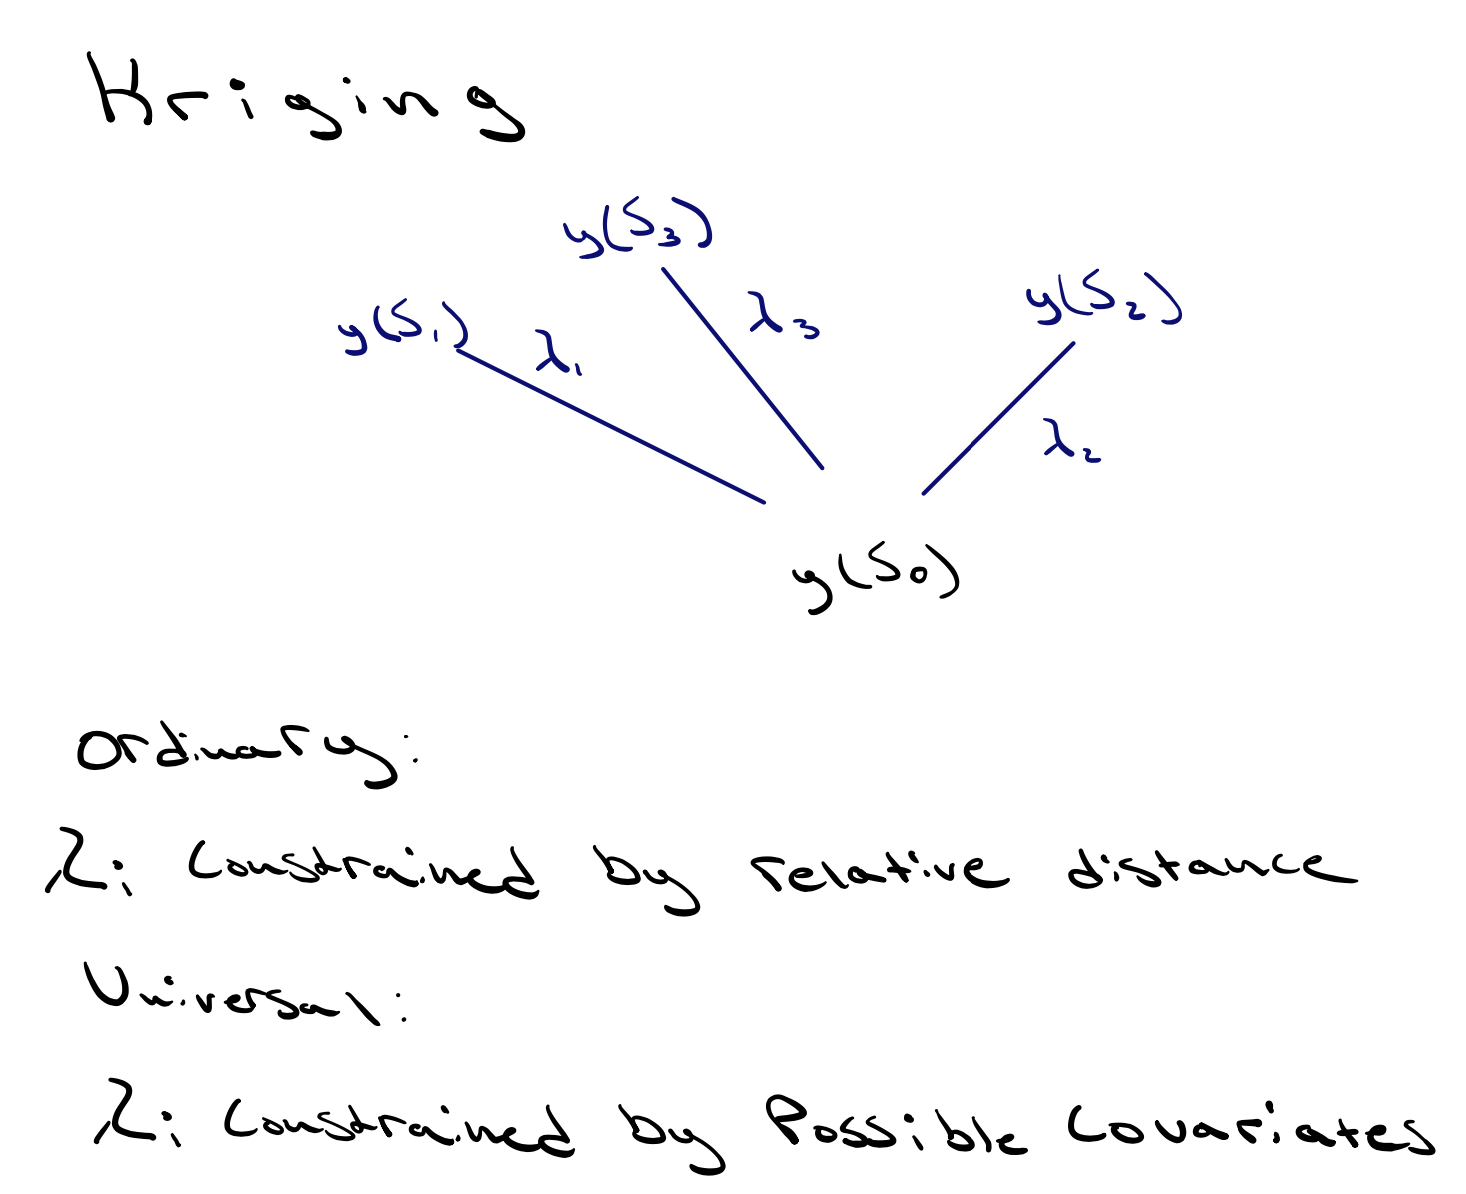
\includegraphics[width = .9\textwidth]{Kriging.png}
    \end{center}
\end{frame}


\begin{frame}{Kriging Overview}
    \begin{center}
    \includegraphics[width = .9\textwidth]{Cokriging.png}
\end{center}
\end{frame}

\begin{frame}{Kriging Overview}
    \begin{center}
    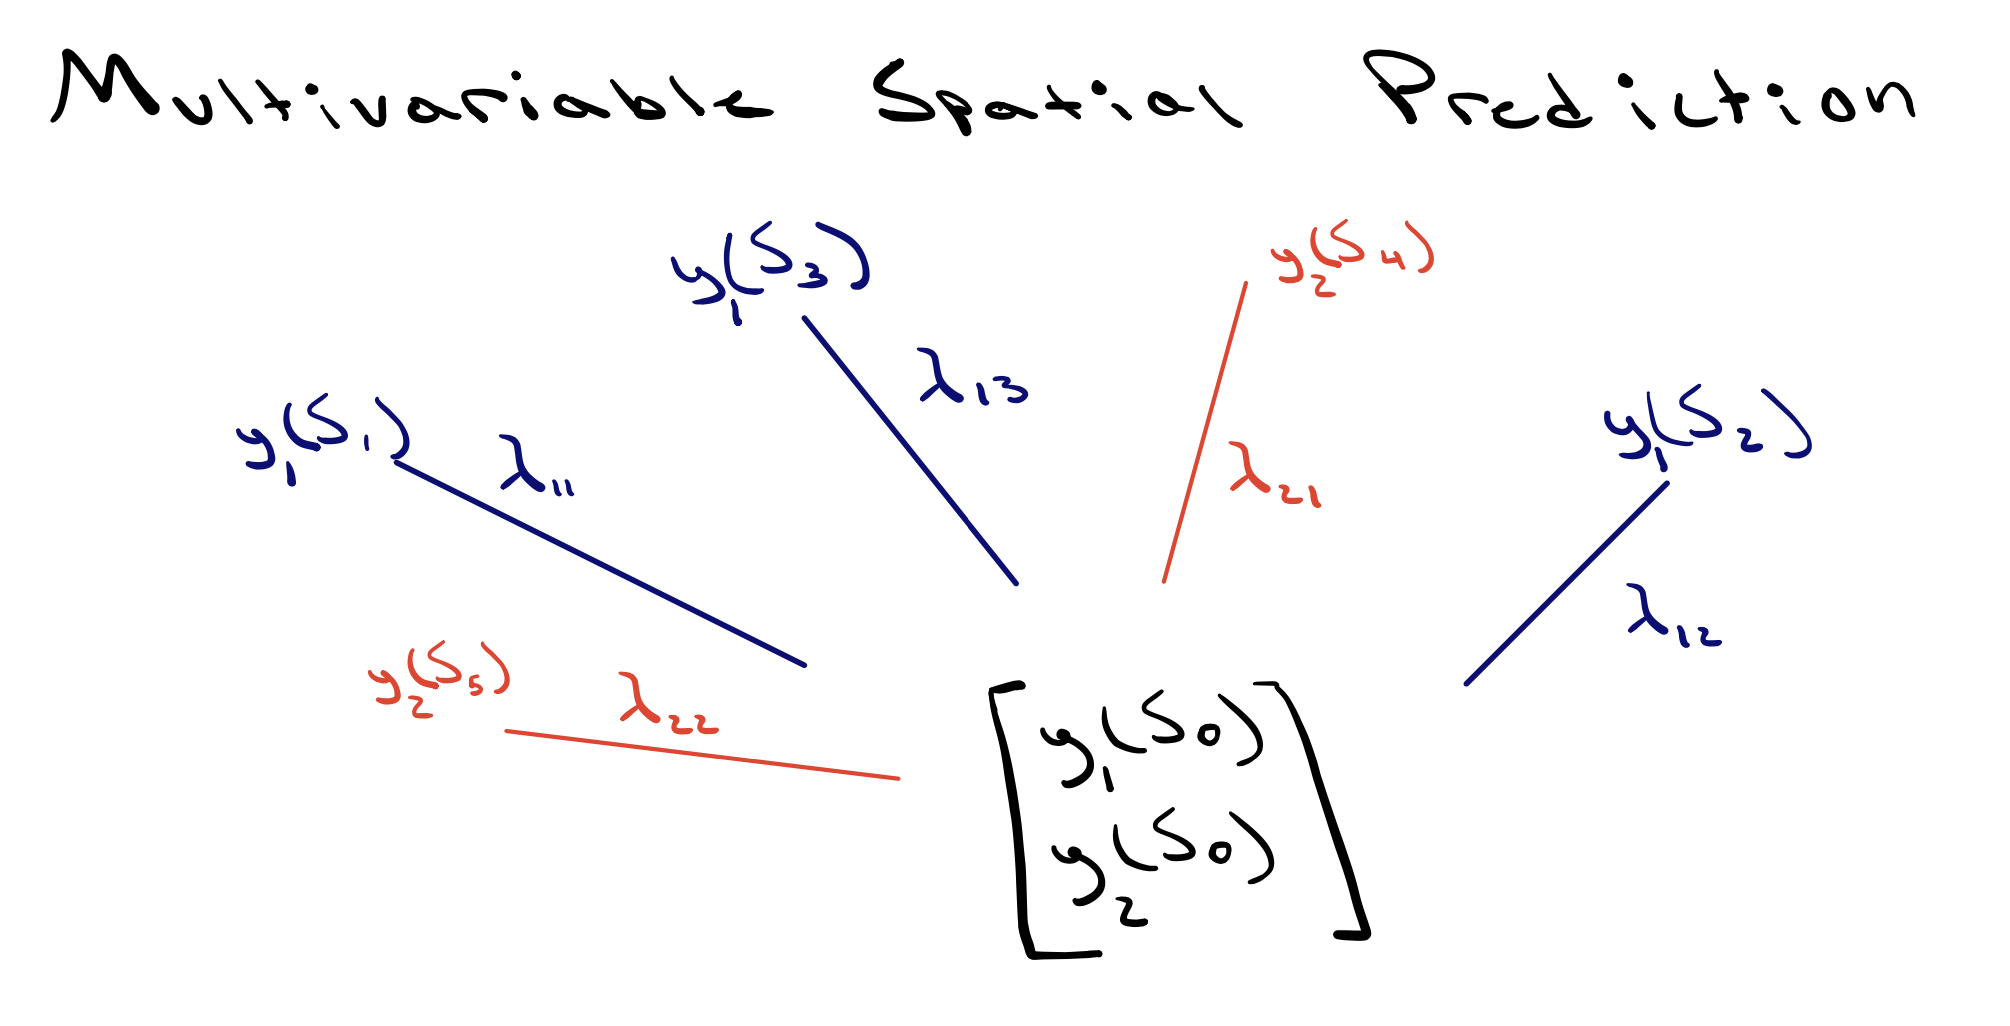
\includegraphics[width = .9\textwidth]{MultivariableSpatialPrediction.png}
\end{center}
\end{frame}


\begin{frame}{Application to Model Validation in Ecology}
    \begin{center}
    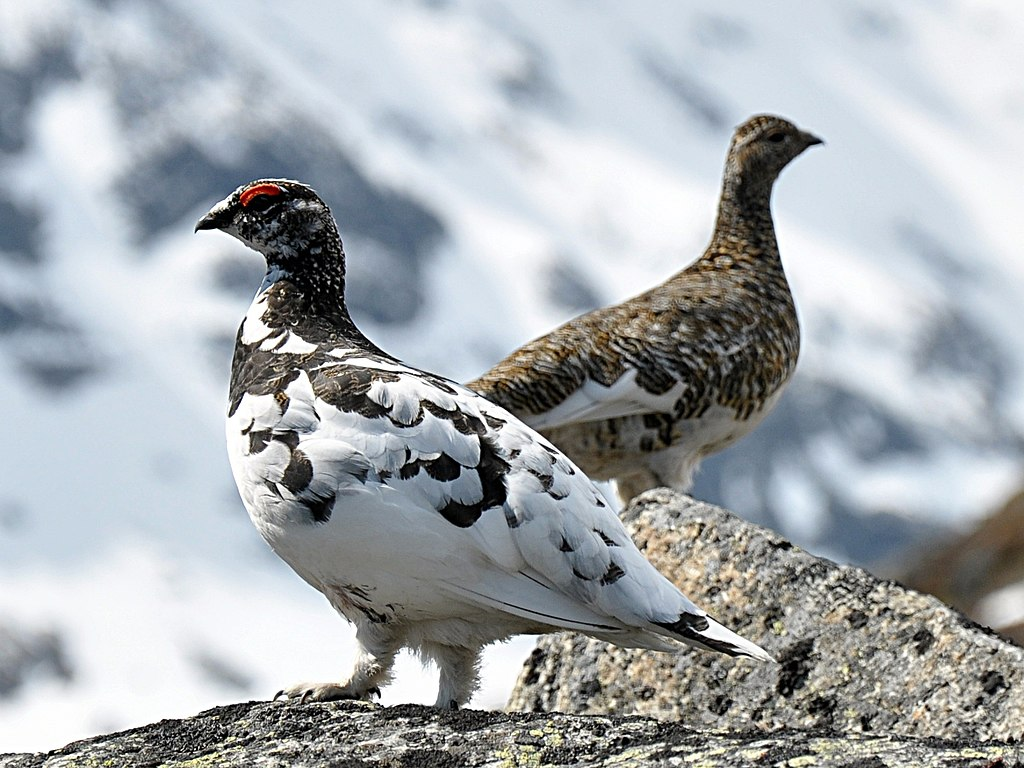
\includegraphics[width = .9\textwidth]{RockPtarmigan.jpg}
\end{center}
\end{frame}

\begin{frame}{Application to Model Validation in Ecology}
    \begin{itemize}
        \item Study put together through several Icelandic environmental agencies, in conjunction with the University of Iceland and the UAF Institute of 
        Arctic Biology. 
        \vfill
        \item Machine learning models (Random Forest and TreeNet) were used to model RIO (relative index of occurrence). 
        \vfill
        \item Nationwide and long term (1860-2021) Rock ptarmigan occurrence data (GBIF). 
        \vfill
        \item Separate occurrence data from the Icelandic Institute of Natural History (2005-2010) for model validation.
         \vfill
        \item 11 Environmental Layers (May, June, July of 2021).
    \end{itemize}
\end{frame}


\begin{frame}{Application to Model Validation in Ecology}
    \begin{center}
        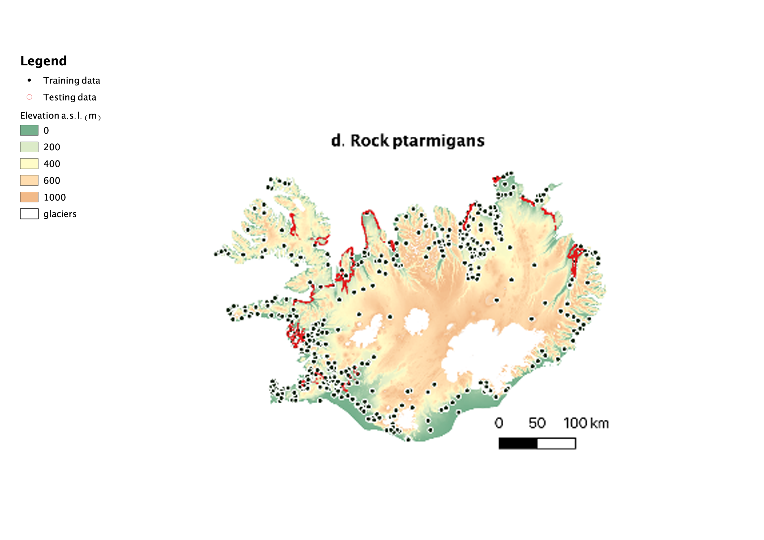
\includegraphics[width = \textwidth]{RockPtarmigan.png}
    \end{center}
\end{frame}


\begin{frame}{}
    \begin{itemize}
        \item Why use Multivariable Spatial Prediction?
    \begin{itemize}
        \item Separate occurrence data does not have the associated predictors (environmental layers).
        \item Current Models are validated with OOB/Cross-Validation.
        \item Temper Expectations.
    \end{itemize}
\end{itemize}
\end{frame}



\begin{frame}{Application to Model Validation in Ecology}
    \begin{itemize}
        \item A tiny bit of code ...
    \end{itemize}
    \begin{center}
        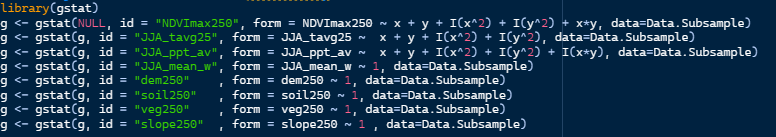
\includegraphics[width = \textwidth]{Code1.png}
    \end{center}
    \begin{center}
        \includegraphics[width = \textwidth]{Code2.png}
    \end{center}
\end{frame}


\begin{frame}{Results}
    \begin{center}
    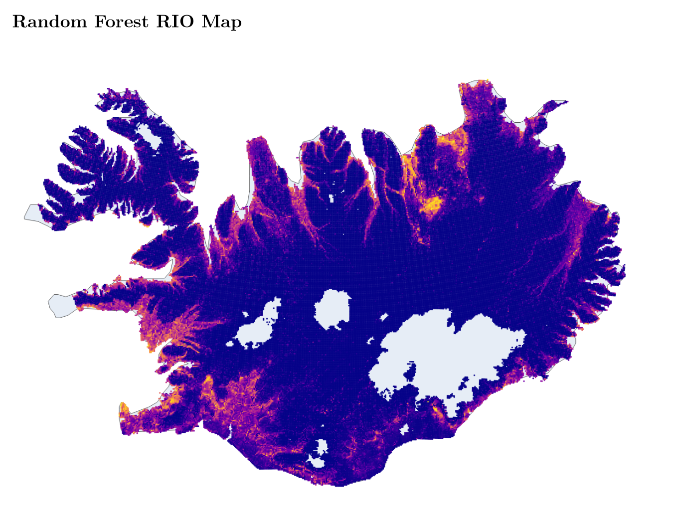
\includegraphics[width = .9\textwidth]{randomforest.png}
    \end{center}
\end{frame}

\begin{frame}{Results}
\begin{columns}[T]
    \begin{column}{.35 \textwidth}
        \begin{itemize}
            \item Accuracy of $91.98\%$ on out of bag samples. 
        \end{itemize}
    \end{column}
    
    \begin{column}{.65\textwidth}
    \begin{center}
        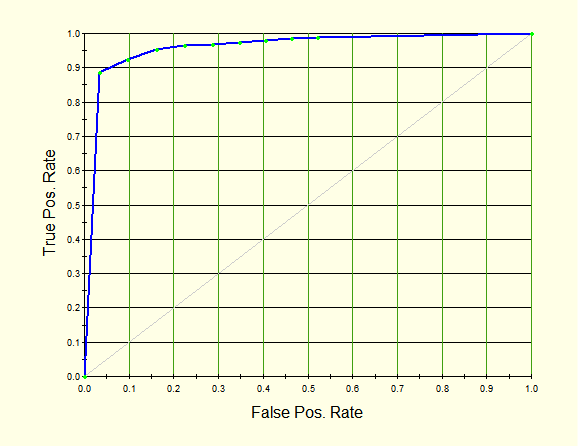
\includegraphics[width = \textwidth]{ROCcurveOOB.png}
    \end{center}
    \end{column}
\end{columns}
\end{frame}

\begin{frame}{Results}
    \begin{columns}[T]
        \begin{column}{.35 \textwidth}
            \begin{itemize}
                \item Accuracy of $72.91\%$ on outside data with kriged predictors.
            \end{itemize}
        \end{column}
        
        \begin{column}{.65\textwidth}
        \begin{center}
            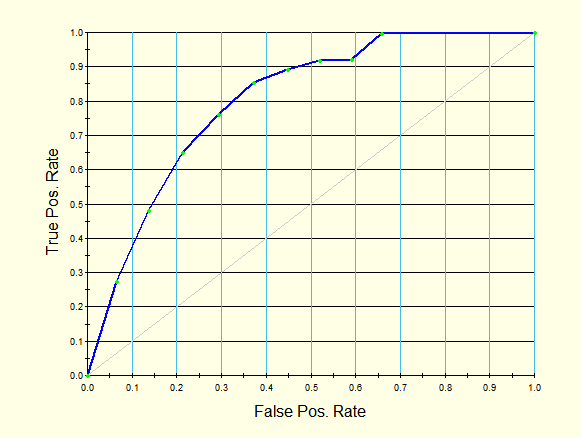
\includegraphics[width = \textwidth]{ROCcurveKriged.png}
        \end{center}
        \end{column}
    \end{columns}
    \end{frame}
\end{document}



\begin{frame}{Results}
    \begin{columns}[T]
        \begin{column}{.35 \textwidth}
            \begin{itemize}
                \item Accuracy of $72.91\%$ on outside data with kriged predictors.
            \end{itemize}
        \end{column}
        
        \begin{column}{.65\textwidth}
        \begin{center}
            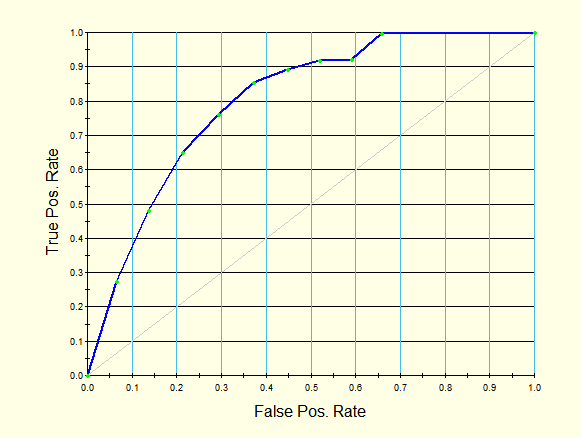
\includegraphics[width = \textwidth]{ROCcurveKriged.png}
        \end{center}
        \end{column}
    \end{columns}
    \end{frame}
\end{document}




## Outline



 - What is Multivariable Spatial Prediction 
     - Building up from kriging, co-kriging we add auxilliary varaibles(covariates), MSP allows covariates and multiple maps or layers. 
     - Technical definition 
     - Examples of Applications in Ecology/GeoSciences. 


- My Project and Data Specifically
     My Project involves mapping the habitability of the rock ptarmgin species accross all of iceland. 
     We used several of these enviornmental layers to create a Relative Index of occourance or habitablity score using
     by predicting presence absence using these enviornmental layers and several decision tree models. 


Introduction: The Goal
 - Applications in Ecology/GeoSciences
Expand the kriging maps into a multivariate dimentsion. 
Many times in ecology/wildlife/Geoscience we are using the massive enviornmental 
layers, regularly spaced data taken from satellites like elevation, land cover, vegitation
or Soil quality. THese things all closely intereact so it would be nice to be able to incorporate 
their connection to enhance our prediction of these layers. 


 - Recall the general outline of regular Kriging

 - Explain the expansion into coKriging

 - Code

 - Application to our data set 

 - results from model validation. 



 land cover classes, soil types, wilderness; and eight
  continuous variables: elevation, Euclidean distance to fenced pastures, 
  Euclidean distance to water (inland), Normalized Difference Vegetation Index (NDVI), 
  slope, as well as average precipitation, temperature and wind speed for June, July and August.


  Predictor variable raster files were tested for multicollinearity 
  using the cor function in the caret package (Kuhn, 2021); none showed a correlation above 0.75.


  Lambert 2016 Icelandic Projection.


  http://fisher.stats.uwo.ca/faculty/kulperger/S9934a/Papers/Pebesma2004.pdf
  https://link.springer.com/content/pdf/10.1007/BF00893273.pdf
  https://upcommons.upc.edu/bitstream/handle/2117/116322/Giraldo,+Delicado+&+Mateu.+2017.+Cokriging+and+multivariate+kriging+methods+based+on+data+of+a+functional+random+field.pdf;jsessionid=0CF25A137AF10296A24C5CD866ACB8BC?sequence=1

  https://petrowiki.spe.org/Kriging_and_cokriging#Cokriging_estimator
